\newpage

%
\textbf{b)} Analizando paso por paso el segundo inciso \ref{b}, se puede resolver en dos partes \textbf{(II $\cap$ III)} y \textbf{(IV' $\cup$ I')} para así unir ambos subconjuntos \\

Resolviendo \textbf{(II $\cap$ III)}

\begin{align*}
(II \cap III)  &= \{ h, j, p, q, r, s  \} \cap \{ a, b, c, d, e, f, g, h, i, j, o, u  \}  \\
  &=   \{ h, j  \}      \\
\end{align*}

Resolviendo \textbf{(IV' $\cup$ I')}

\begin{align*}
(IV' \cup I')  &=  \{ a, b, c, d, e, i, o, t, u, v, w, x, y, z \}  \cup \{ b, c, d, f, g, h, j, k, l, m, n, p, q, r, s, t, v, w, x, y, z \}  \\
  &=  \{ a, b, c, d, e, f, g, h, i, j, k, l, m, n, o, p, q, r, s, t, u, v, w, x, y, z \} \\
\end{align*}

Juntando ambos lados para armar (II $\cap$ III) - (IV' $\cup$ I'):

\begin{align*}
(II \cap III) - (IV' \cup I') &= \{ h, j  \} - \{ a, b, c, d, e, f, g, h, i, j, k, l, m, n, o, p, q, r, s, t, u, v, w, x, y, z \} \\
  &= \{ \} 
\end{align*}

Por lo tanto el resultado es un subconjunto vacío:

\begin{equation*}
    \boxed{(I - I') \cup (III' \cap II)' = \{  \} }
\end{equation*}





Para obtener el diagrama de Venn, se puede hacer por partes, el lado derecho y lado izquierdo, quedando: \\

\textbf{(II $\cap$ III)}: 

\begin{figure}[htbp]
\centering
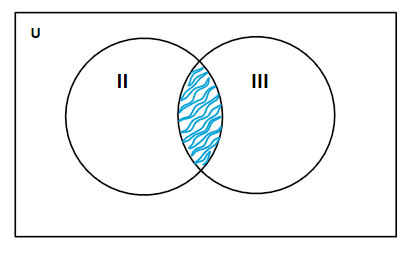
\includegraphics[width=8cm]{b/aa.png}
\caption[]{Diagrama de Venn de (II $\cap$ III)}
\end{figure} 

\newpage

\textbf{(IV' $\cup$ I')}:

\begin{figure}[htbp]
\centering
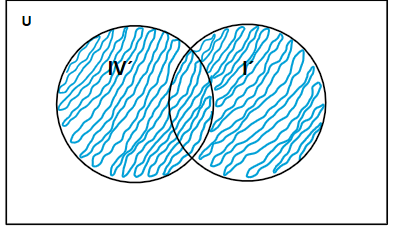
\includegraphics[width=8cm]{b/bb.png}
\caption[]{Diagrama de Venn de (IV' $\cup$ I')}
\end{figure} 

Sacando la diferencia, (II $\cap$ III) - (IV' $\cup$ I'), queda que no existe ningún diagrama representativo, ya que es un subconjunto vacío



